\graphicspath{{./gui/Bilder/}}

\chapter{Arbeitspaket GUI}
Für die Analyse, den Entwurf, die Implementierung dieses Arbeitspaketes übernahm Herr Krause die Verantwortung, wobei er bei der Implementierung von den selbst erstellten Steuerelementen vom Herrn Krupinski unterstützt wurde. Während der Integration des Arbeitspaketes waren die Herren Krupinski und Schleinkofer unterstützend beteiligt.
\paragraph{}
In der Projektspezifikation wurde die Anforderung der Visualisierung von Motor-Charakteristiken und die Steuerung des Motors mit aufgenommen. Zu diesem Zweck wurde eine Benutzeroberfläche in der Programmiersprache C\# mit Hilfe des Grafik-Framework\footnote{Rahmenstruktur in der Software} \textit{WPF} \footnote{Windows Presentation Foundation} von Microsoft erstellt.

\section{Analysephase}
Das Arbeitspaket GUI wurde mit einer Analysephase begonnen. In dieser Phase wurden die möglichen Funktionalen und Nicht-Funktionalen Anforderungen in einer Spezifikation zusammengetragen und aufgelistet. Es wurden Stakeholder\footnote{Projektbeteiligte, welche nicht an der Entwicklung beteiligt sind} befragt, um die gewünschten Anforderungen an das System zu erhalten und anschließend wurden die Ergebnisse der Befragung validiert, priorisiert und in die Spezifikation mit aufgenommen. Die umzusetzenden Projektinhalte wurden dann aus dieser abgleitet.\\
Die wichtigsten drei Anforderungen jeder Gruppe, basierend auf der Analyse:\\

\begin{minipage}[t]{0.5\textwidth}
\textbf{Funktionale Anforderungen:}
\begin{itemize}
	\item Anzeige von Sensordaten in der GUI
	\item Einstellung möglicher Parameter des Motors
	\item Justierung der PID Regelung in der GUI
	\end{itemize} 
\end{minipage}\begin{minipage}[t]{0.5\textwidth}
\textbf{Nicht-Funktionale Anforderungen:}
\begin{itemize}
	\item Die Software soll Modular aufgebaut und erweiterbar sein
	\item Es soll das aktuelle Metro-Design verwendet werden
	\item Der Aufbau soll möglichst einfach gehalten sein, um die Stabilität und Benutzbarkeit zu verbessern.
\end{itemize} 
\end{minipage}
\newline
\newline
\newline
Als weiteres Ergebnis der Analyse ergab sich eine zwingende Abhängigkeit zu dem Arbeitspaket Kommunikation, wo die erforderlichen Schnittstellen und Datenstrukturen in enger Zusammenarbeit erstellt wurden. Diese sind ebenfalls in die Spezifikation mit aufgenommen worden.

\section{Entwurfsphase}
Mit den Ergebnissen der Analysephase, wurde ein Entwurf der Benutzeroberfläche erstellt. Dieser wurde auf der einen Seite für die Code Struktur und Architektur durchgeführt, auf der anderen Seite wurden mögliche Designentwürfe des Layouts erstellt.\\

Als grundlegende Architektur wurde ein drei Schichtenmodell\ref{fig:arc} verwendet, welches den Anforderungen der Analysephase gerecht wird und allen Entwicklern des Projektes bekannt ist. In diesem gewählten Modell kommunizieren nur benachbarte Schichten miteinander. Und jede Schicht hat eine separate Aufgabe.

\begin{figure}[h]
	\centering
		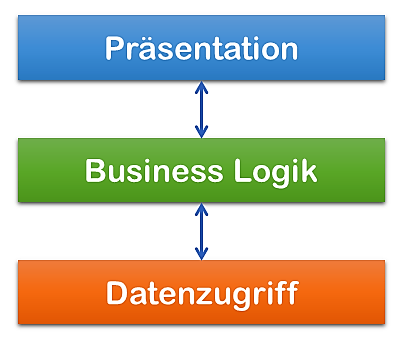
\includegraphics[scale=0.5]{Arc1}
		\caption{Grober Architektur Entwurf}
		\label{fig:arc}
\end{figure}

Es wurden mehrere Entwurfsmuster verwendet, welche zur Softwarequalität beitragen und dem Entwickler einzelne Lösungsgerüste für wiederkehrende Probleme liefern.
\\
Für die oberen beiden Schichten wurde das MVVM\footnote{kurzw. für Model-View-ViewModel} Entwurfsmuster\ref{fig:mvvm} gewählt. Dieses Muster trennt die Oberfläche von der zugrundeliegenden Business-Logik, dies ermöglicht es die Komponenten unabhängig und austauschbar von der Businesslogik zu entwickeln.\\ 

\begin{figure}[h]
	\centering
		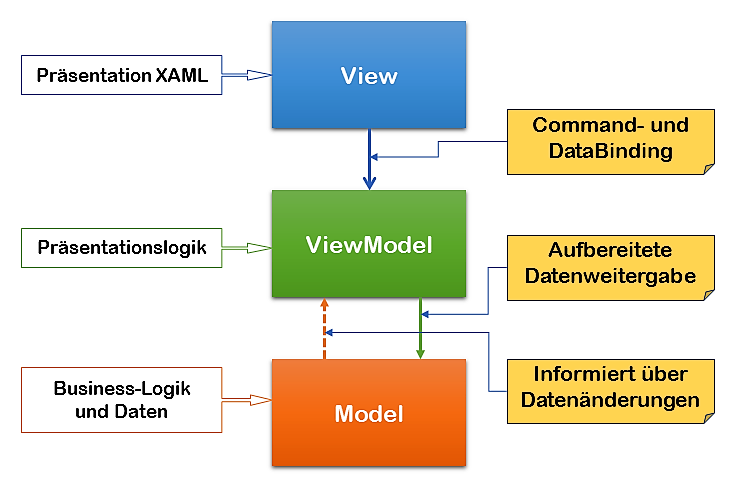
\includegraphics[width=0.6\textwidth]{MVVM}
		\caption{MVVM-Konzept}
		\label{fig:mvvm}
\end{figure}

Weitere eingesetzte Entwurfsmuster sind das Kommandomuster, welches alle ausgeführten Events auf der Benutzeroberfläche auffängt und im ViewModel behandelt und verarbeitet, das Repository\footnote{engl. Haufen}-Muster, welches die Daten Verwaltung und Kommunikation zu Subsystemen übernimmt und flexible auf Änderungen im Kommunikationsmodul reagiert und das "Umkehrung der Kontrolle"-Muster, für dessen Zweck ein Abhängigkeits-Container zu beginn des Systemstarts erstellt und mit allen bekannten Abhängigkeiten gefüllt wird. Anschließend ist der Zugriff auf die im Container befindlichen Objekte von jedem Punkt der Anwendung her ermöglicht.\\

Wie bereits in der Analysephase erwähnt, wurden die Datenstrukturen dem Kommunikationsmodul angepasst siehe Abbildung \ref{lst:SensorData}.\\
\begin{lstlisting}[frame=single, caption=Beschreibung der Sensordatenstruktur, label=lst:SensorData]
    public class SensorData
    {
        public ulong Timestamp { get; set; }
        public SortedList<ushort, double> DataTable { get; set; }
    }
\end{lstlisting}
Im zweiten Teil des Entwurfes wurde ein erstes einfaches Layout\ref{fig:gui} erstellt. Für dieses wurde das Werkzeug Pencil\footnote{Link zum Projekt \url{http://pencil.evolus.vn/}} eingesetzt. Es ist einfach zu bedienen und lieferte schnell ein Ergebnis, welches im Projektteam besprochen werden konnte.

\begin{figure}[h]
	\centering
		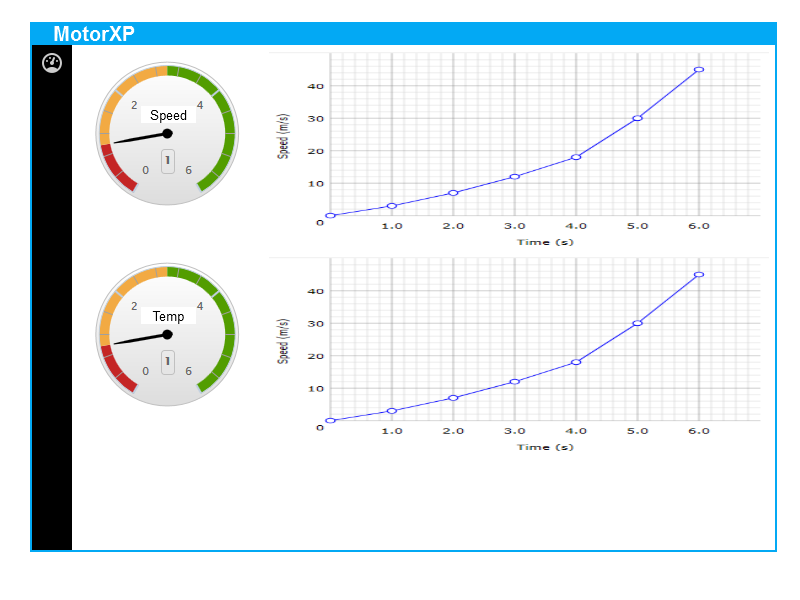
\includegraphics[width=0.5\textwidth]{Mockup}
		\caption{Erster Layout Entwurf der GUI}
		\label{fig:gui}
\end{figure}


\section{Implementierung}
In diesem Abschnitt werden wurden die Ergebnisse der Entwurfsphase umgesetzt und die Benutzeroberfläche erstellt. Das Programm wurde mit dem Visual Studio 2015 in der Programmiersprache C\# und den .NET Framework WPF erstellt. In dieser Phase kommen die vom Herrn Krupinski erstellten Steuerelemente zum Einsatz unterstützt.\\

Zu beginn der Implementierung wurde die Frage aufgeworfen, welche Technologie für die Oberfläche zum Einsatz gebracht werden sollten. Zur Auswahl stand, es mit neuesten Multi-Plattform fähigen Web-Technologien umzusetzen und auf das ASP.NET-Framework\footnote{Microsoft Framework zur Entwicklung von Web-Applikationen} zu setzen oder eine reine Desktop Applikation mit dem WPF-Framework umzusetzen. Aufgrund des relativ knappen Zeitplanes für das Projekt und der mehrheitlichen Erfahrungen im WPF-Framework, wurde sich für dieses entschieden.\\

Als Entwicklungsumgebung wurde das Visaul Studio Enterprise 2015 eingesetzt. Dieses Tool bietet dem Entwickler einen sehr kraftvollen Code-Editor, einfach zu bedienenden Debugger, umfangreiche Diagnose Tools, integriertes Test Framework und ist flexibel erweiterbar zusätzlich werden Projekt Templates bereitgestellt, welche schon grundlegende Konzepte wie Architektur Muster mitbringen.\\

Als Grundlage für den Start des Projektes wurde das MVVM-Light\footnote{Link zum Projekt\url{https://mvvmlight.codeplex.com/}} Toolkit verwendet. Es beinhaltet grundlegende Funktionalitäten und Templates, welche den Entwickler, indem es Basistechnologien wie die Architektur Struktur MVVM und DI-Techniken mitbringt, entlasten. Dieses Toolkit ist ebenfalls als Erweiterung direkt im Visual Studio verfügbar.\\

Der Datenzugriff wurde durch den Einsatz vom Repository-Muster (siehe Abbildung \ref{fig:repo}) realisiert. Dies ermöglichte zu beginn des Projektes und für Test gegen eine Attrappe des Kommunikationsmoduls zu entwickeln. Diese täuschte das fehlende Modul vor und konnte problemlos durch das fertig implementierte Modul ersetzt werden. Durch die vorangegangene Schnittstellen Definition mussten für die Integration des Kommunikationsmoduls keine Änderungen an der internen Systemlogik vorgenommen werden.   

\begin{figure}[h]
	\centering
		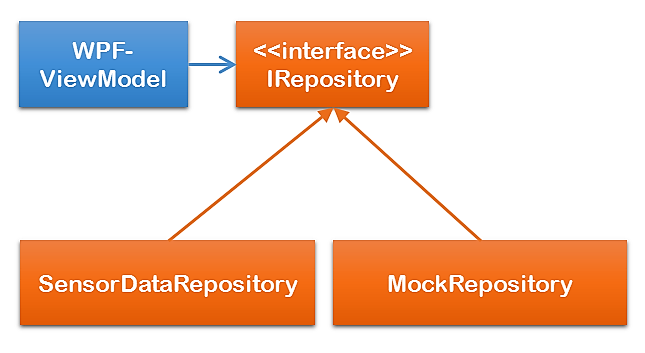
\includegraphics[width=0.5\textwidth]{RepoPattern}
		\caption{Repository Muster in der GUI}
		\label{fig:repo}
\end{figure}

Ein weiteres Problem, welches es zu lösen gab, waren die Steuerelemente für die Anzeige. Es folgte eine kurze Evaluation und Testphase für die möglichen Tachometer und Linienchart Anzeigen, leider mit dem Ergebnis, dass die fertigen Produkte entweder Kostenpflicht waren oder schlecht dokumentiert und nicht genügend Anpassbar für unseren Zweck waren.\\

Darauf hin erstellte der Herr Krupinski diese beiden aufwändigen Steuerelemente als Benutzerdefinierte WPF-Steuerelemente selbst, welche uns die geforderten Funktionalitäten und die notwendige Veränderbarkeit mitbrachten. 

\subsubsection*{Gauge Control}
Das entwickelte "Gauge"\footnote{engl. Tachometer} Control in Abbildung \ref{fig:gauge} besteht aus einer Skala(1) mit einem minimal und maximal Wert, einen Zeiger(2) und einem Label(3), welches den Aktuellen Wert anzeigt.

\begin{figure}[h]
	\centering
		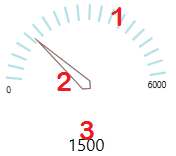
\includegraphics[width=0.3\textwidth]{Gauge1}
		\caption{Tachometer Anzeige der GUI}
		\label{fig:gauge}
\end{figure}

\subsubsection*{LineChart Control}

In Abbildung \ref{fig:line} ist das "LineChart"\footnote{engl. Liniendiagramm} Control abgebildet. Es besteht aus einem anzeige Raster(1), einen Graphen(2) zur Visualisierung der Werte einer Anzeige für die Y-Achse(3) mit einstellbaren Werten und einer Anzeige für den ersten und letzten Wert der X-Achse(4).

\begin{figure}[h]
	\centering
		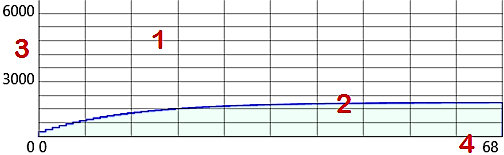
\includegraphics[width=0.6\textwidth]{Line1}
		\caption{Liniendiagramm Anzeige der GUI}
		\label{fig:line}
\end{figure}


Diese Steuerelemente bieten dem Entwickler diverse Einstellmöglichkeiten in Form und Farbgebung und sind beliebig erweiterbar für kommende Anforderungen.\\

Die beiden Benutzer definierten Steuerelemente wurden zu einem eigenen Control zusammengefasst und mit weiteren Steuerelementen ergänzt. In Abbildung \ref{fig:control1} ist exemplarisch ein komplettes Anzeigeelement für einen Sensorwert abgebildet.

\begin{figure}[h]
	\centering
		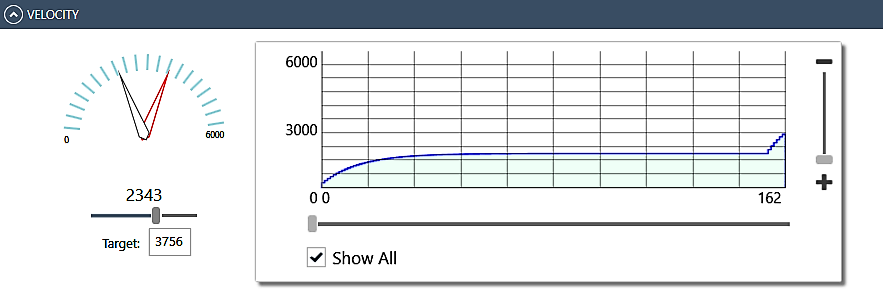
\includegraphics[width=\textwidth]{GUIScreenshot3}
		\caption{Datenanzeige Control}
		\label{fig:control1}
\end{figure}

Die Abbildung \ref{fig:guifinal} zeigt fertige die GUI zum Ende des Projektes. Sie ist aktuell in der Lage die definierten Sensorwerte anzuzeigen, die einzelnen Anzeigeelemente\ref{fig:control1} bieten die Möglichkeiten im Liniendiagramm zu Zoomen und das Wertefenster der X-Achse festzulegen und zu verschieben. Für einstellbare Größen, wie zum Beispiel die Drehgeschwindigkeit kann ein Zielwert eingegeben werden, welcher durch eine zweite rote Nadel im Tachometer angezeigt wird. Im oberen Bereich der GUI kann man die Regelparameter ebenfalls verändern und an den Controller senden.

\begin{figure}[h]
	\centering
		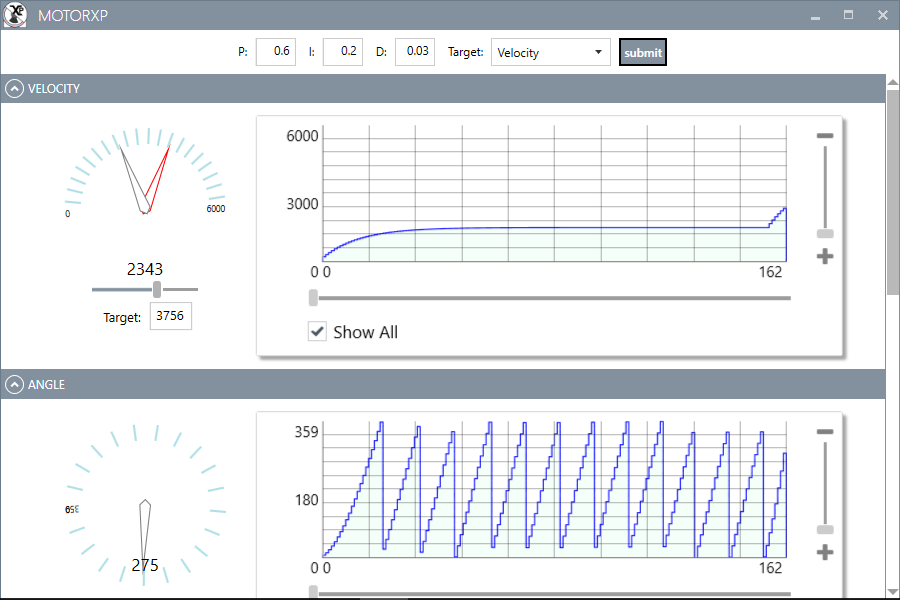
\includegraphics[width=\textwidth]{GUIScreenshot2}
		\caption{Ansicht der GUI zum Projektende}
		\label{fig:guifinal}
\end{figure}


Zum Abschluss der Implementierungsphase wurden Unit-Tests geschrieben, wodurch noch einige Fehler aus der Codebasis aufgespürt werden konnten. Diese Test helfen ebenfalls zukünftigen Entwickler an dem Projekt, da unbedachte Änderungen welche zu Fehlverhalten der Applikation führen können schnell aufgedeckt werden.

\section{Ausblick}
Dieser Abschnitt beinhaltet mögliche Erweiterungen und nicht vollständig umgesetzte Projektteile, welche eine weitere Gruppe als Arbeitspaket aufnehmen kann. 

\begin{description}


\item[Multi-Platformfähigkeit] Durch die Separierung der einzelnen Codeteile in eigenständige Projekte und die strikte Umsetzung eines Domain Driven Designs kann man die WPF GUI austauschbar machen und durch zum Beispiel eine Web-API ersetzen, welche anschließend mit einem Web-Frontend z.B. ASP.NET oder Angular2 kommuniziert. Auch eine Smartphone Applikation mit zum Beispiel Xamarin wäre möglich.

\item[MouseHover in LineChart] Diese Funktionalität konnte leider nicht Fertiggestellt werden, es wird noch nicht der aktuelle Wert unter der Maus angezeigt.

\item[Änderung des Layoutes] Durch eine Änderung des Layoutes wäre es möglich alle Sensorwerte auf einen Bildschirm Darzustellen, ohne die Notwendigkeit von Scrolbars zu haben. Empfehlung dafür wäre ein Wrappanel mit Horizontaler Ausrichtung.

\item[Hall Pattern Anzeige] Die Aktuelle Anzeige des Hall Pattern ist in einem extra Control unter dem ItemsTemplate für die Anzeigeelemente, dies verhindert Aktuell die einfache Umsetzung der vorher beschriebenen Änderung des Layouts. Hier müsste das Hall Pattern mit in das ItemsTemplate implementiert werden.

\item[Auswahl des Com-Ports] Eine wichtige Erweiterung wäre eine Einstellmöglichkeit für den Com-Port, da dieser aktuell Hardcoded ist und ggf. im Quelltext angepasst werden muss. Eine Notlösung wäre eine Auslagerung der Einstellung in eine Konfigurations-Datei. Aber die Bessere Lösung wäre eine ComboBox in der GUI zur Auswahl aus verfügbaren Ports. 

\item[Mehrere Inputs] Die GUI könnte noch für mehrere Inputs erweitert werden um es zu ermöglichen mehrere Messstationen oder die Simulation nebeneinander Vergleichend laufen zu lassen.

\item[Benutzer Handbuch] Dem knappen Zeitrahmen geschuldet wurde noch kein Benutzerhandbuch erstellt. Dies wäre Sinnvoll nach der Änderung des Layouts zu erstellen, um aktuelle Bilder verwenden zu können.

\item[Weitere Tests] Sinnvoll für mehr Stabilität wären weitere Tests, einmal für die CustomControls (Gauge und LineChart) Unittests, für die Oberfläche allgemein Coded-UI Tests und ein automatisierter Integrationstest für das Kommunikationsmodul.

\item[Import/Export] Eine Im-/Exportfunktion um Testläufe zu sichern und wiederholt zu laden.

\item[RingSpeicher] Implementierung eines Ringspeichers, welcher eine Maximale Anzahl an Elementen fasst und überschüssige Daten auf der Festplatte oder ähnlich Speichert, um ein Überlaufen des Arbeitsspeichers zu verhindern.

\end{description}

